% It is an example file showing how to use the 'sigkddExp.cls' 
% LaTeX2e document class file for submissions to sigkdd explorations.
% It is an example which *does* use the .bib file (from which the .bbl file
% is produced).
% REMEMBER HOWEVER: After having produced the .bbl file,
% and prior to final submission,
% you need to 'insert'  your .bbl file into your source .tex file so as to provide
% ONE 'self-contained' source file.
%
% Questions regarding SIGS should be sent to
% Adrienne Griscti ---> griscti@acm.org
%
% Questions/suggestions regarding the guidelines, .tex and .cls files, etc. to
% Gerald Murray ---> murray@acm.org
%
 
\documentclass{sigkddExp}

\usepackage{booktabs} 
\usepackage{multirow, array}
\usepackage{makecell}
\usepackage[table,x11names]{xcolor}
\usepackage{color}
\usepackage{enumitem}
\usepackage{soul}
\usepackage{tabularx}
\usepackage[skip=1ex]{caption}

\begin{document}

%
% --- Author Metadata here ---
% -- Can be completely blank or contain 'commented' information like this...
%\conferenceinfo{WOODSTOCK}{'97 El Paso, Texas USA} % If you happen to know the conference location etc.
%\CopyrightYear{2001} % Allows a non-default  copyright year  to be 'entered' - IF NEED BE.
%\crdata{0-12345-67-8/90/01}  % Allows non-default copyright data to be 'entered' - IF NEED BE.
% --- End of author Metadata ---

\title{6.864, Fall 2017 - Neural Approaches to Question Retrieval}
\subtitle{Codebase: https://github.com/shashank-srikant/6.864\_term\_project}

% You need the command \numberofauthors to handle the "boxing"
% and alignment of the authors under the title, and to add
% a section for authors number 4 through n.
%
% Up to the first three authors are aligned under the title;
% use the \alignauthor commands below to handle those names
% and affiliations. Add names, affiliations, addresses for
% additional authors as the argument to \additionalauthors;
% these will be set for you without further effort on your
% part as the last section in the body of your article BEFORE
% References or any Appendices.

\numberofauthors{2}
%
% You can go ahead and credit authors number 4+ here;
% their names will appear in a section called
% "Additional Authors" just before the Appendices
% (if there are any) or Bibliography (if there
% aren't)

% Put no more than the first THREE authors in the \author command
%%You are free to format the authors in alternate ways if you have more 
%%than three authors.

\author{
%
% The command \alignauthor (no curly braces needed) should
% precede each author name, affiliation/snail-mail address and
% e-mail address. Additionally, tag each line of
% affiliation/address with \affaddr, and tag the
%% e-mail address with \email.
\alignauthor Vadim Smolyakov*\\
       \affaddr{CSAIL, MIT}\\
       \email{vss@csail.mit.edu}
\alignauthor Shashank Srikant\titlenote{Author order decided by tossing a fair coin.}\\
       \affaddr{CSAIL, MIT}\\
       \email{shash@mit.edu}
}

\balancecolumns
\date{30 July 1999}
\maketitle
\begin{abstract}
Content on the internet grows at an exponential rate. Given this growth, finding relevant information accurately becomes a critical task for the NLP community to address. More so, with this rapid growth, curating labeled datasets to build models for the available wide variety of content has become extremely time and resource intensive. In this work, we explore whether neural models are able to successfully model content similarity and retrieval tasks, and whether they can transfer knowledge from one domain, where supervised labels are available, to a domain with no such labels. Specifically, we explore content similarity in online discussion forums, where we explore the following questions - a. how effectively can neural approaches model question-answer retrieval tasks. Given a question and answer pair present on an online discussion forum, such a retrieval task finds similar pairs on that forum. b. Given a model of question-answer similarity in one online discussion forum, how effective are neural approaches in transferring that knowledge to a new, loosely related domain. In this work, we explore a baseline approach of modeling question similarity tasks on the popular Stack Exchange online community \textit{Ask Ubuntu}. We show how neural architectures like LSTMs and CNNs outperform traditional approaches in information retrieval. Additionally, and importantly, we explore the problem of transferring these models to detect question-answer similarity on \textit{Android Stack Exchange},  a similar yet different online discussion community where members troubleshoot Android related problems. We show how neural domain adaptation techniques successfully beat baseline transfer techniques. We also discuss some limitations and challenges in using such architectures.
\end{abstract}

\begin{table*}[th]
\begin{tabular*}{\linewidth}{m{0.13\linewidth}m{0.12\linewidth}m{0.18\linewidth}m{0.18\linewidth}m{0.28\linewidth}}
\toprule
\toprule
\textbf{Scenario} & \textbf{Setting} & \textbf{Nature of Data} & \textbf{Learning Paradigm} & \textbf{Main Concepts}  \\
\toprule 
 \makecell{$\mathcal{D}_S = \mathcal{D}_T,$\\$ \mathcal{T}_S = \mathcal{T}_T$}
& Traditional Machine learning
& Labelled data in source domain(s) and unlabeled data in target domain
& Source and target domains are exactly the same
& Learn models on training set and test on future unseen data \\
\cmidrule{1-5}
 \multirow{2}{\linewidth}{\textbf{\makecell{$\mathcal{D}_S \neq \mathcal{D}_T$,\\ $\mathcal{T}_S = \mathcal{T}_T$}}} 
& \multirow{2}{\linewidth}{Transductive Transfer Learning}
& \multirow{2}{\linewidth}{Labelled data in source domain(s) and unlabeled data from $\mathcal{P}(X_S) \neq \mathcal{P}(X_T$)}
& \textbf{Single source domain adaptation}
%\cellcolor{blue!25}
& Learning common shared representation; instance weighing, parameter transfer
\\
\cmidrule{4-5}
 
&
&
& Multi-source adaptation
& Classifier combination; efficient combination of information from multiple sources; Feature representation \\
\cmidrule{1-5} 

\multirow{2}{\linewidth}{No conditions on $\mathcal{D}_S$, $\mathcal{D}_T$, 
but $\mathcal{T}_S \neq \mathcal{T}_T$ }
& \multirow{2}{\linewidth}{Inductive Transfer Learning}
& Unlabeled data in source domain(s) and labeled data in target domain
& Self-taught learning
& Extracts higher level representations from unlabeled auxiliary data to learn instance-to-label mapping with labeled target instances
\\
\cmidrule{3-5} 
& & Labeled data is available in all domains
& Multi-task learning
& Simultaneously learns multiple tasks within (or across) domain(s) by exploiting the common feature subspace shared across the tasks \\
\cmidrule{1-5}
\makecell{$\mathcal{D}_S\neq \mathcal{D}_T$\\$\mathcal{T}_S \neq \mathcal{T}_T$}
& Kim et al., 2015 \cite{kim2015new}
& Labeled data in source and target domains
& Transfer learning with disparate label set
& Disparate fine grained label sets across domains, however, same coarse grained labels set can be invoked across domains
\\
\bottomrule
\end{tabular*}
\caption {A brief summary of different transfer learning approaches. $\mathcal{D}$ is the domain and $\mathcal{T}$ is the task. The boldfaced cell highlights the approach explored in this work. This summary is based on the work detailed in the survey paper by Pan et. al.\protect\cite{pan2010survey}}
\label{tab:related_work}
\end{table*}

\section{Introduction}
The problem of text similarity, and specifically, similarity of short queries or answers found on the internet, have been central to the modern NLP community. With the explosion in content on the internet, a lack of robust tools to find similar content has the risk of creating further similar and redundant content, which only exacerbates the original problem.

Another relevant and pressing concern which such an explosion and variety of content has introduced is the increased cost of building predictive NLP, NLU models which cater to such content. The variety in content requires building a model from scratch, irrespective of how closely related the content may have been to a previously built model. For instance, if we were to model the reviews written for movies, we would have to reinvest effort and time in modeling reviews written for another domain, say, food or hotels. In spite there being conceptual, semantic similarities between the tasks of reviewing movies and reviewing food, models have to be created anew. And each such modeling exercise demands a large repository of curated, preferably labeled data, which most often is not feasible to put together. The pressing challenge such a variety of content has created is to be able to learn with minimal supervision, and from loosely related datasets.

In this work, we investigate two problems - one, to model question-similarity tasks using state of the art techniques in neural modeling and two, transfer those models to a loosely related, yet equally rich domain, under the constraint of having no supervised information on that new domain. Specifically, we explore the problem of finding similar question-answer pairs on the popular \textit{Ask Ubuntu Stack Exchange}.\footnote{https://askubuntu.com} This discussion forum focuses on troubleshooting queries on Ubuntu, the popular open-source operating system. In addition to  learning models to find relevant question-answer pairs on this forum, we also use this domain to transfer knowledge onto modeling question-answer similarity in \textit{Android Stack Exchange}.\footnote{https://android.stackexchange.com} This is an online community, similar in setup and structure to \textit{Ask Ubuntu}, wherein short queries and corresponding answers on Android-related troubleshooting are present.

In this work, we investigate how state of the art neural architectures for NLP applications perform on the task of question similarity. Traditionally, text similarity tasks were solved using information retrieval techniques like building an indexer and applying string search over the indexed corpus. A lot of variations to this general strategy have been explored over the years. We study how more recent techniques like RNNs and CNNs, which have shown to successfully model a variety of NLP tasks, solve the question retrieval problem. For the domain adaptation task, we explore adversarial training techniques \cite{ganin2015unsupervised, lei2015semi} as well as the performance on different architectures like $\textsf{Doc2Vec}$ \cite{doc2vec1} and Siamese neural networks \cite{siamese}.

This study demonstrates the relevance of neural techniques in a critical NLP task like question-answer retrieval. We demonstrate how using neural approaches, one can outperform traditional information retrieval techniques while not having to invest heavily in engineering the right features to get to such performance. Additionally, we show the successful transfer of domain knowledge from one domain to another using state of the art neural transfer techniques.

This work is organized into the following sections - Section \ref{related} discusses related work in this field. Sections \ref{in_domain}, \ref{domain_adapt},  \ref{other_techniques} discuss various techniques to model in-domain and domain adaptation tasks for the given problem. Section \ref{experiments} discusses the experiment setup and the results. Section \ref{discussion} concludes our work.


\begin{table*}[ht]
\centering
\begin{tabularx}{\linewidth}{XX}
    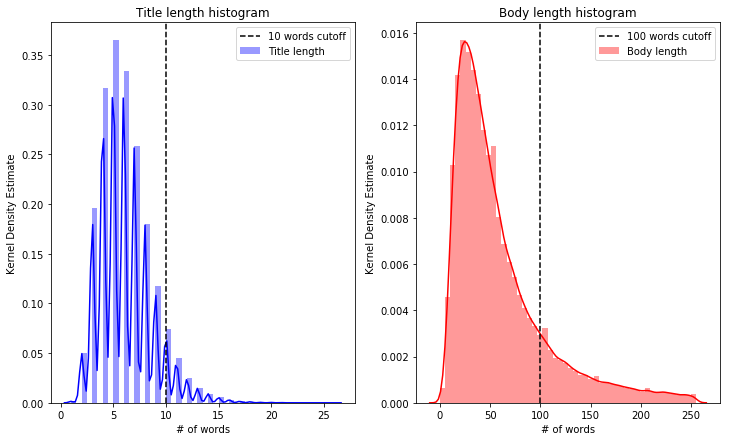
\includegraphics[width=\columnwidth]{img/hist_dataset1} 
    \captionof{figure}{\textit{Ask Ubuntu} dataset description}
    \label{fig:his1}
    
&   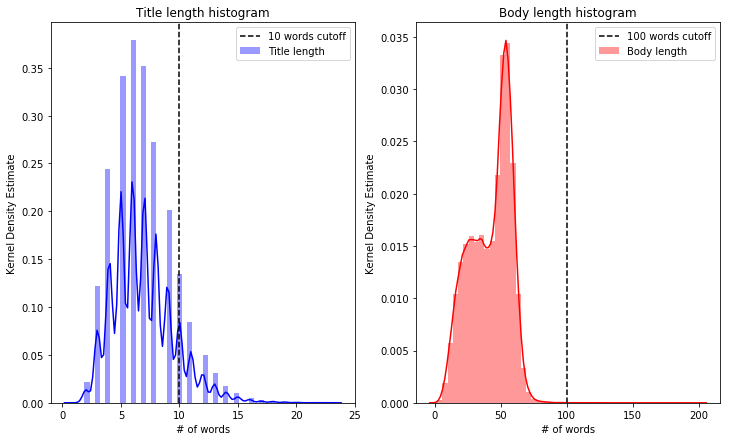
\includegraphics[width=\columnwidth]{img/hist_dataset2}
    \captionof{figure}{\textit{Android} dataset description}
    \label{fig:his2}
    \\
   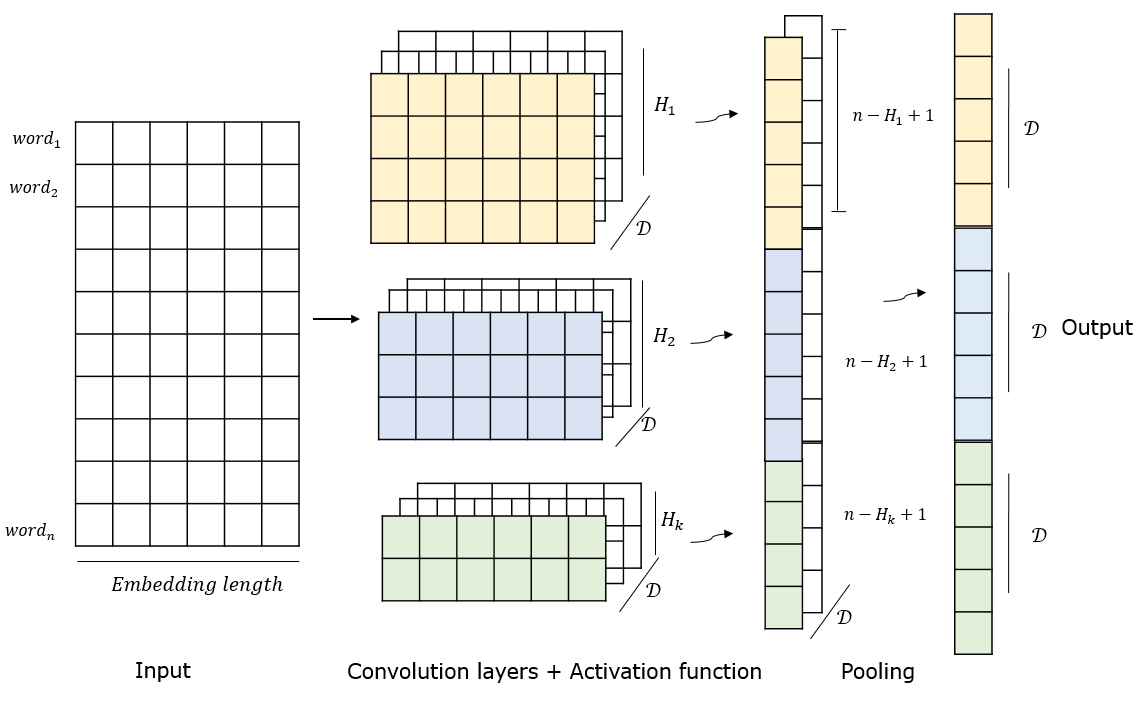
\includegraphics[width=\columnwidth]{img/cnn}
   \captionof{figure}{CNN architecture}
   \label{fig:cnn}
   
&  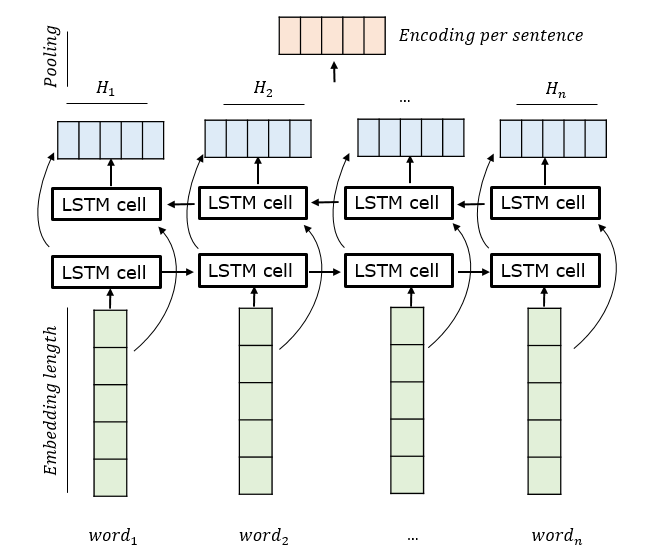
\includegraphics[width=\columnwidth]{img/lstm}
   \captionof{figure}{LSTM architecture}
   \label{fig:lstm}
\end{tabularx}
\end{table*}

\section{Related work}
\label{related}
Given the growing popularity of community QA forums, question retrieval has emerged as an important area of research. Recent work has also gone beyond word-based methods to represent this task. For instance, Feng et. al. \cite{feng2015applying} learn word embeddings using category-based metadata information for questions. They define each question as a distribution which generates each word (embedding) independently, and subsequently use a Fisher kernel to assess question similarities. Dos Santos et. al. \cite{dos2015learning} propose an approach which combines a convolutional neural network (CNN) and a bag of words representation for comparing questions. In contrast to \cite{feng2015applying}, Lei et. al. \cite{lei2015semi} treat each question as a word sequence as opposed to a bag of words, and apply recurrent CNNs instead of traditional CNNs. We base our work on \cite{lei2015semi}. We apply different off-the-shelf deep learning models to encode a meaningful embedding and define similarity over these embeddings.

Domain adaptation has been an active area of research in NLP. Table \ref{tab:related_work}  summarizes different settings of transfer learning \cite{pan2010survey}. Our work explores techniques in unsupervised domain adaptation, where the source and target domains ($\mathcal{D}$) are different, but share a common task ($\mathcal{T}$) to achieve. The summary helps in understanding where our approach lies in this spectrum of techniques.

We study in this work the scenario where the domains vary while the tasks remain the same. This is referred to as transductive transfer learning. This is the most extensively studied settings in the transfer learning literature and can be broadly categorized as single and multi-source adaptation. Single source adaptation\cite{chen2009extracting, ando2005framework, daume2009frustratingly} primarily aims at minimizing the divergence between the source and target domains either at instance or feature levels. The general idea being identifying a suitable low dimensional space where transformed source and target domains data follow similar distributions and hence, a standard supervised learning algorithm can be trained.

Multiple methods perform unsupervised domain adaptation by matching the feature distributions in the source and the target domains. Some approaches perform this by reweighing or selecting samples from the source domain  \cite{borgwardt2006integrating, huang2007correcting, gong2012geodesic}, while others seek an explicit feature space transformation that would map source distribution into the target ones \cite{pan2011domain, gopalan2011domain, baktashmotlagh2013unsupervised}. An important  aspect of the distribution matching approach is the way the (dis)similarity between distributions is measured. Here, one popular choice is matching the distribution means in the kernel-reproducing Hilbert space \cite{borgwardt2006integrating, huang2007correcting}, whereas \cite{gong2012geodesic, fernando2013unsupervised} map the principal axes associated with each of the distributions. The approach explored in this work is based on \cite{ganin2015unsupervised} and also attempts to match feature space distributions. However, this is accomplished by modifying the feature representation itself rather than by reweighing or geometric transformation. Also, the method used to measure the disparity between distributions based on their separability is implicitly different and is done by a deep discriminatively-trained classifier in our work as.


\section{In-domain Question similarity}
\label{in_domain}
We first explore the task of question similarity by training a domain-specific classifier. The domain we have explored in this work involves the questions and answers asked on \textit{Ask Ubuntu}. The dataset for this task was curated by \cite{lei2015semi}. 

\begin{table}[h]
\begin{tabular}{l|r|r}
     
     & $\mathsf{source} (\mathcal{D_S})$
     & $\mathsf{target} (\mathcal{D_T})$
     \\
     \toprule
     Description
     & \textsf{AskUbuntu}
     & \textsf{Android SE}
     \\
     Total \# of questions
     & 167763
     & 42970
     \\
     Avg words/title (std dev)
     & 6 (2.5)
     & 9 (3.9)
     \\
     Avg words/body (std dev)
     & 92 (210.6)
     & 69 (24.1)
     \\
     \# unique queries in train-set
     & 12724
     & NA
     \\
     \# unique queries in test-set
     & 200
     & 1148
     
\end{tabular}
\caption{Summary statistics of our dataset}
\label{tab:dataset}
\end{table}

\subsection{Dataset}
We describe here the dataset that we base our work on.
\begin{itemize}[topsep=0pt,itemsep=-1ex,partopsep=1ex,parsep=1ex]
\item The \textit{Ask Ubuntu} dataset consists of questions and answers related to problems people face in Ubuntu, the Linux operating system
\item Each query has two components - a title and main body. The average title length is 6 words and the average body length is 92 words long after removing stop-words. Figure \ref{fig:his1} shows the distribution of word lengths
\item Each query is associated with a few ($<10$) positive (similar) questions and $100$ randomly drawn questions from the corpus which serve as negative (dissimilar) questions.
\item The dataset contained a total of $167$K questions. Of these, $12724$ were used as queries to train on.
\item Each query-positive and query-negative pair is also associated with its $\mathsf{BM25 scores}$ provided by Apache Lucene. This served as a baseline in our experiments.
\end{itemize}

\subsection{Model}
We model the task of in-domain question similarity in the following manner
\begin{itemize}[topsep=0pt,itemsep=-1ex,partopsep=1ex,parsep=1ex]
  \item We define a word-level deep neural network (DNN). The network takes a sequence of indices corresponding to word embeddings. We average the title and the body of each query, and use the averaged representation to compute similarity.
  \item We use word embeddings pre-trained on source domain and the Wikipedia.
  \item To train the classifier to find similar and dissimilar questions for a given query, we associate each query with two sets of texts - the set of similar questions as marked by users on \textit{Ask Ubuntu}, and 100 randomly sampled questions from the corpus which serve as dissimilar pairs. The user-defined questions are used only during training. Since user-marked similar questions are not comprehensive and serve only as a weak proxy, the system is tested on expert-marked similar questions.
  \item We use cosine similarity to rank similar questions by computing the cosine of the angle between the query encoding and its associated candidate question.
  \item We use a max-margin framework for learning parameters $\theta$ of our network. Specifically, in a context of a particular training example where $q_i$ is paired with $p^+_i$, we minimize the max-margin loss $L(\theta)$ defined as\\
  \begin{equation}
  \max_{p^- \in Q(q_i)} \{s(q_i,p^-;\theta) - s(q_i,p^+_i;\theta) + \delta(p, p^+_i)\}
  \end{equation}
where $\delta(.,.)$ denotes a non-negative margin. We set $\delta(p, p^+_i)$ to be a small constant when $p \neq p^+_i$ and 0 otherwise. The parameters $\theta$ can be optimized through sub-gradients ${\partial L}/{\partial \theta}$ aggregated over small batches of the training instances \cite{lei2015semi}.
  \item The neural network essentially serves as an encoder to generate a representation in a low-dimension space.
  \item We compare performance on two neural network architectures: Long Short-Term Memory (LSTM) Recurrent Neural Network (RNN) and a Convolutional Neural Network (CNN).
  \item Similarity is evaluated on standard information retrieval metrics like \textit{Precision@1}, \textit{Precision@5}, \textit{Mean Average Precision}, and \textit{Mean Reciprocal Rank}. The inputs to each of these metrics is a ranked list of scores. We pass in the cosine similarity scores obtained between the query and each of the positive and negative questions associated with that query, as our ranked list. The $\mathsf{BM25 scores}$ for each of these pairs is used as a baseline similarity score and their evaluations on the metrics mentioned above are considered the baseline performance indicators for this approach.
\end{itemize}

\subsection{CNN}
Figure \ref{fig:cnn} illustrates the CNN architecture implemented in this work. We detail the inputs to the different layers of the network here.
We define a CNN with the following layers -
\begin{itemize}[topsep=0pt,itemsep=-1ex,partopsep=1ex,parsep=1ex]
\item \textbf{Input vector $\mathbf{X}$} of dimensions: ($\mathbf{B}$, $\mathbf{W}$) ($\mathbf{B}$: batch size, $\mathbf{W}$: max \# of words in sentence in batch)
\item \textbf{Embedding layer} Looks up word embeddings of indices in $\mathbf{X}$. Resulting dimension: ($\mathbf{B}$, $\mathbf{W}$, $\mathbf{D}$) ($\mathbf{D}$: \# of embeddings per word)
\item \textbf{Convolution, tanh} A convolution layer and then through tanh is applied to $\mathbf{X}$. Resulting dimension: ($\mathbf{B}$, $\mathbf{K}$, $\mathbf{Y}$)($\mathbf{K}$: Depth of filter, i.e. \# of filters of given height, $\mathbf{Y}$: \# of values sliding the filter over the input)
\item \textbf{Pooling} Mean pooling of convolution layers. Resulting dimension: ($\mathbf{B}$, $\mathbf{K}$)
\item The resulting encoded embedding of dimension ($\mathbf{B}$, $\mathbf{K}$) for $\mathbf{B}$ words in a given batch.
\end{itemize}

\subsection{LSTM}
Figure \ref{fig:lstm} illustrates the LSTM architecture implemented in this work. We detail the inputs to the different layers of the network here.
\begin{itemize}[topsep=0pt,itemsep=-1ex,partopsep=1ex,parsep=1ex]
\item \textbf{Input vector $\mathbf{X}$} of dimensions: [$\mathbf{B}$, $\mathbf{W}$, $\mathbf{D}$], where $\mathbf{B}$ is the batch size, $\mathbf{W}$ is max number of words, and $\mathbf{D}$ is the embedding dimension
\item \textbf{Embedding layer} Looks up word embeddings of indices in $\mathbf{X}$.
\item \textbf{LSTM layer} returns the hidden state and LSTM cell state.
\item \textbf{Pooling} Average pooling is used to average the outputs of the bi-directional LSTM producing a summary vector of dimension [$\mathbf{B}$, $2\times \mathbf{H}$], where $\mathbf{H}$ is the hidden size. 
\end{itemize}


\section{Domain Adaptation (DA)}
\label{domain_adapt}
 We use adversarial training techniques \cite{ganin2015unsupervised} to adapt to a domain having no labeled data, having trained a model on a domain with labeled data. In this section and the next, we describe the dataset we worked on, the architecture for the adversarial model we use, and other models for DA we tried.


\subsection{Dataset}
We worked with two datasets, one as our $\mathsf{source}$ domain, wherein we had labeled data and another as our $\mathsf{target}$ domain, where we had no labeled data. The task on both these datasets was the same - to predict similarity between questions. The $\mathsf{source}$ domain in our experiments was the \textit{AskUbuntu} dataset, described in the previous section. The $\mathsf{target}$ domain was the \textit{Android Stack Exchange}, a question-answering site on Android-related issues. Table \ref{tab:dataset} describes the summary statistics of this dataset. No training set was available for this dataset - all questions were divided into validation and test sets. Each query was again associated with a few ($<10$) positive and $100$ negative questions. These were expert-annotated. The final model was tested on 1148 unique queries.

\subsection{Model}
We model this task of unsupervised domain adaptation using a neural adversarial approach \cite{ganin2015unsupervised}. The core idea is as follows - 
\begin{itemize}[topsep=0pt,itemsep=-1ex,partopsep=1ex,parsep=1ex]
    \item We define an encoder which takes in data from the $\mathsf{source}$ domain and learns a representation which predicts the similarity for tasks in its own domain, given that we have labels for this domain. This is similar to the in-domain learning described in the previous section. We refer to this network as the \textit{encoder network} here on.
    \item While the primary goal of predicting $\mathcal{Y}_\mathsf{source}$ remains, we define an adversarial objective to guide the direction of the embeddings encoded by the encoder network in a way to make them abstract enough to be able to discriminate $\mathcal{Y}_\mathsf{target}$ as well.
    
    \item We do this by setting up another network to learn this adversarial objective. We refer to this network as \textit{adversarial network} here on. We set the goal of the adversarial network to predict whether a given data-point input to it originates from either the $\mathsf{source}$ or $\mathsf{target}$ dataset. The idea behind setting up this objective is that if the origin of the input data is being discriminated well by the adversarial network, then the features are still specific enough to discriminate between the two datasets. What we want is to however have an abstract enough feature space which, in spite of predicting the labels of the $\mathsf{source}$ well, is unable to distinguish between the $\mathsf{source}$ and $\mathsf{target}$ dataset.
    \item The objective of the adversarial network is set up in a way to propagate a negative weight to the encoder whenever it successfully discriminates between $\mathsf{source}$ and $\mathsf{target}$. This ensures the successful transfer of the encoded embeddings to the $\mathsf{target}$ domain. Figure \ref{fig:adversarial} depicts this arrangement.
    
    \item  Specifically, let $\theta_f$ be the parameters of the question encoder (generator) $G_f$ and $\theta_d$ be the parameters of the domain classifier (discriminator). The loss objective then is defined as:
    \begin{equation}
    \left.\begin{aligned}
     \min E(\theta_f, \theta_d) &= \sum_{i=1}^{n}L_{y}^{i}(\theta_f) - \lambda^{t}\sum_{i=1}^{n}L_{d}^{i}(\theta_f, \theta_d)
     \\
     \end{aligned}\right.
     \end{equation}
     
    \begin{equation}
    \left.\begin{aligned}
     &= \sum_{i=1}^{n}L_y(G_f(x_i;\theta_f), y_i) 
      - \lambda^{t} \sum_{i=1}^{n}L_d(G_d(G_f(x_i;\theta_f), \theta_d), y_i)
    \end{aligned}\right.
    \end{equation}
    where $L_y(\theta_f)$ is the multi-margin loss and $L_d(\theta_f, \theta_d)$ is the binary cross-entropy loss. During adversarial training, we jointly minimize the multi-margin loss and maximize cross-entropy loss. We accomplish this with a single back-propagation step by minimizing the total loss $E(\theta_f, \theta_d)$ and reversing the gradient of the domain classifier during the weight update, e.g. by setting a negative learning rate.
\end{itemize}


\begin{figure}[h]
\centering
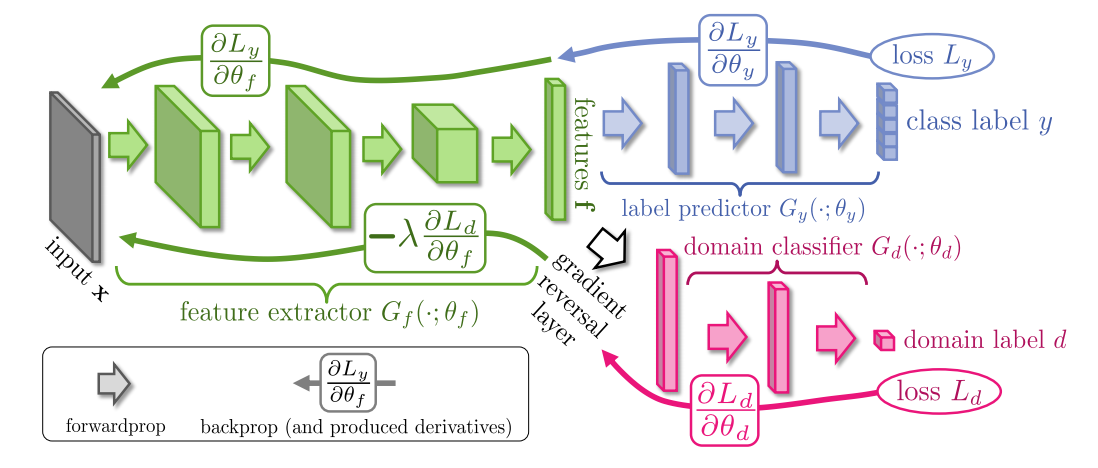
\includegraphics[width=\columnwidth]{img/adversary}
\caption{Adversarial network for unsupervised domain adaptation investigated in this work. Image source: Ganin et al., 2015 \protect\cite{ganin2015unsupervised}}
\label{fig:adversarial}
\end{figure}
 
\begin{table}[h]
\centering
\begin{tabularx}{\columnwidth}{X}
    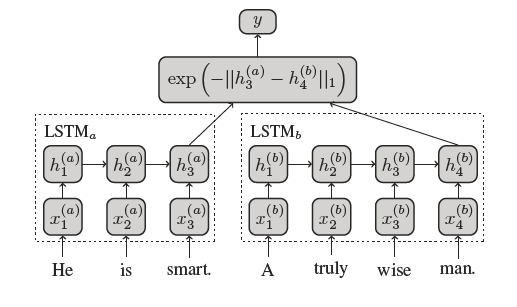
\includegraphics[keepaspectratio, width=\columnwidth]{img/siamese_architecture}
    \captionof{figure}{Siamese RNN. Image source: Neculoiu et al. \protect\cite{siamese}}
   \label{fig:siamese}
   \\
    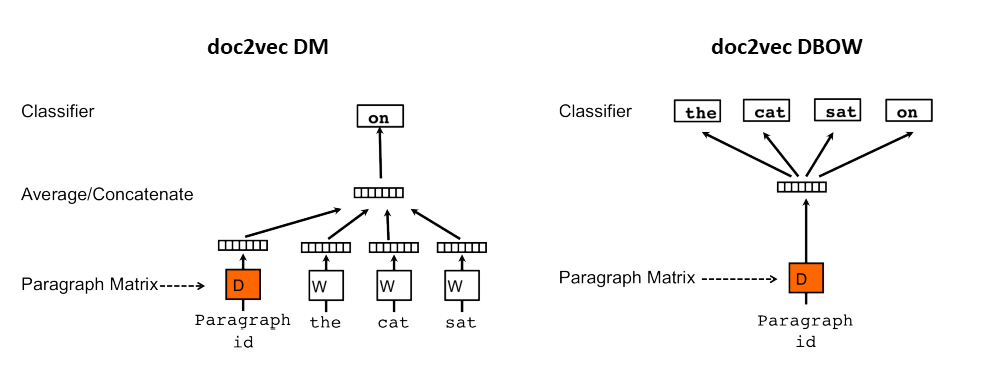
\includegraphics[width=\columnwidth]{img/doc2vec_architecture}
    \captionof{figure}{Doc2Vec. Image source: Le et al. \protect\cite{doc2vec1}}
    \label{fig:doc2vec}
\end{tabularx}
\end{table}

\section{Exploring Domain Adaptation}
\label{other_techniques}
We explored two other techniques to carry out unsupervised domain transfer - $\textsf{doc2vec}$ \cite{doc2vec1} and Siamese recurrent networks \cite{siamese}. We describe each briefly here:
\begin{itemize}[topsep=0pt,itemsep=-1ex,partopsep=1ex,parsep=1ex]

\item \textbf{Siamese RNN} 
 Siamese neural networks \cite{siamese} are characterized by shared weights and are trained with a \textit{contrastive loss function} that differentiates the inputs. They are thus well-suited for computing similarity between a query and a candidate question. We use a shared bi-directional LSTM as an input encoder and add several fully connected layers for domain adaptation. The architecture is shown in Figure \ref{fig:siamese}. The contrastive loss function $L(x_1,x_2,y)$ is defined as
\begin{eqnarray}
L &=& \frac{1}{2}(1-y)D_{w}^{2} + \frac{1}{2}y \max \{0, -D_w + \Delta\}^{2} \\
D_w &=& \sqrt{[RNN(x_1) - RNN(x_2)]^2}
\end{eqnarray}
where $y$ is a binary label equal to $0$ for similar inputs (in which case we want to minimize the distance $D_w$) and equal to $1$ for dissimilar inputs (in which case we want to maintain a margin $\Delta$). The distance $D_w$ is a pairwise Euclidean distance between RNN encodings of the inputs $x_1$ and $x_2$. In order for the Siamese RNN to generalize to domain adaptation, we include dropout\cite{srivastava2014dropout} in between the dense layers with keep probability equal to $0.5$. Alternatively, \textit{variational dropout}\cite{kingma2015variational} can be used to tune the keep probability to improve generalization performance.

\item \textbf{$\textsf{doc2vec}$} A \textsf{doc2vec} model was proposed by Le and Mikolov \cite{doc2vec1} as an extension of word2vec to learn fixed-length feature representations from variable-length pieces of texts, such as sentences, paragraphs, and documents. Thus, each document is represented by a dense vector which is trained to predict words in the document. While the word vectors represent the concept of a word, the document vector intends to represent the concept of a document. There are two doc2vec architectures: Distributed Memory (DM) and Continuous Bag of Words (CBOW) as shown in Figure \ref{fig:doc2vec}. The DM model acts as memory that remembers what is missing from the current context. The CBOW model samples a text window, then samples a random word from the text window and forms a classification task of predicting the random word given the text window. Such a document vector representation can likely model both domains in a domain-adaptation task.
\end{itemize}


\begin{table}[b]
\begin{tabularx}{\columnwidth}{l|r|l|r}
      \multicolumn{2}{c|}{\textbf{CNN direct}}
     & \multicolumn{2}{c}{\textbf{LSTM direct}}
     \\
     \toprule
     \textbf{Parameter}
     & \textbf{Value}
     & \textbf{Parameter}
     & \textbf{Value}
     \\
     \midrule
     Kernel size
     & [1-5] $\times$ 200
     & Hidden size
     & 128 $\times$ 2
     \\
     Output channels
     & 5$\times$200
     & Loss margin
     & 0.4
     \\
     Weight decay
     & 1e-5 
     & Weight decay
     & 1e-5 
     \\
     Learning rate
     & 1e-3
     & Learning rate
     & 1e-3
     \\
     Loss margin
     & 0.4
     & Bidirectional
     & True
     \\
     Pooling
     & average
     & Pooling
     & average
     \\
     Batch size
     & 32
     & Batch size
     & 32
\end{tabularx}
\caption{Optimal hyperparameters of the direct transfer CNN and LSTM networks - Experiment 1}
\label{tab:param_direct}
\end{table}

\section{Experiments and Results}
\label{experiments}
We pose the following research questions, whose answers we investigate in this work
\begin{itemize}[topsep=0pt,itemsep=-1ex,partopsep=1ex,parsep=1ex]
\item \textbf{E1:} How well do deep neural encoders such as LSTM and CNN solve the task of in-domain question retrieval. How do they compare to baselines and the state of the art? What are the limitations?
\item \textbf{E2:} How effective are deep adversarial neural methods in adapting from one domain to another to learn a common task. How do they compare to baselines and the state of the art? What are the limitations?
\item \textbf{E3:} How well can a Siamese neural network architecture and $\mathsf{doc2vec}$ model question-similarity tasks and whether they aid in domain adaptation.
\end{itemize}

\subsection{Experiment 1}
To answer $\mathbf{E1}$, we measure the performance of our neural encoders against a baseline of $\mathsf{BM25}$ scores provided for each query in the test set of the corpus. These scores are pre-computed for each query-positive and query-negative pair. The ranked list of these scores per query is used as a baseline performance on the four metrics we choose (see Section \ref{in_domain} for details on the metrics).

\textbf{Implementation specifics:}
In our implementation, we ensure that stop words are removed from the corpus. This reduces the average sentence length by 30\%. Each input in a batch that we pass to our network consists of words in a query, one positive question corresponding to it and all its corresponding negative questions.  We represent unseen words in the pre-trained embeddings with an all-zero vector. We equate sentence length in a batch by padding with $0$s till maximum length of the batch. The 0-padding is taken into account while mean pooling the intermediate results in the network. We do not train the pre-trained embedding layer. In this work, to limit computational requirements, we consider only the first 10 words in the title and the first $100$ words in the body of each sentence. Further, we score only $40$ random negative questions per query instead of the full $100$ provided in the dataset. All hyperparameters are tuned on the dev set. The number of trainable network parameters are constrained to a budget of $450K$ parameters so that the expressability of the models are comparable. Table \ref{tab:param_direct} lists the various hyperparameters of the encoder network. The model is trained on 12K queries and tested on 2K queries. Words not seen during training are treated as 0-vectors. All experiments were carried out on a CUDA-enabled GTX Titan GPU. Each model was run for 16 training epochs, averaging to $15$ min/epoch for LSTM and $10$ min/epoch for CNN.

\textbf{Results:}
Table \ref{tab:exp1} tabulates the performance of neural encoders on the task of question retrieval and similiarity. We compare ranking performance of CNN and LSTM models against $\textsf{BM25}$ based ranking by Apache Lucene. Higher number indicates higher performance. We also record the number of trainable parameters used. We analyze and discuss these results in Section \ref{discussion}.
\begin{table}[h]
    \begin{tabular}{l|r|l|r}
          \multicolumn{2}{c|}{\textbf{CNN adversarial}}
         & \multicolumn{2}{c}{\textbf{LSTM adversarial}}
         \\
         \toprule
         \textbf{Parameter}
         & \textbf{Value}
         & \textbf{Parameter}
         & \textbf{Value}
         \\
         \midrule
         $\lambda$
         & 1e-6
         & $\lambda$
         & 1e-7
         \\
          Weight decay
         & 1e-5 
         & Weight decay
         & 1e-5 
         \\
         Learning rate
         & 1e-3
         & Learning rate
         & 1e-3
         \\
         Discriminator
         & 4-layer MLP
         & Discriminator
         & 4-layer MLP
         \\
         Output channels
         & 1250
         & Hidden size
         & 128
         \\
         Kernel size
         & [2-6] x 250
         & Bidirectional
         & False
         \\
         Embed dim
         & 300
         & Embed dim
         & 300
         \\
         Pooling
         & average
         & Pooling
         & average
         \\
         Batch size
         & 32
         & Batch size
         & 32
    \end{tabular}
    \caption{Optimal hyperparameters of the adversarial CNN and LSTM networks - Experiment 2.}
    \label{tab:param_adversarial}
\end{table}


\begin{table}[b]
 \begin{tabular}{l|r|l|r}
          \multicolumn{2}{c|}{\textbf{Siamese RNN}}
         & \multicolumn{2}{c}{\textbf{\textsf{doc2vec DM/DBOW}}}
         \\
         \toprule
         \textbf{Parameter}
         & \textbf{Value}
         & \textbf{Parameter}
         & \textbf{Value}
         \\
         \midrule
         Hidden size
         & 128
         & \textsf{doc2vec} dim
         & 256
         \\
         Bi-directional
         & True
         & Context window
         & 10
         \\
         Dropout prob
         & 0.5
         & Min count
         & 2
         \\
         Loss margin
         & 0.5
         & Learning rate
         & 0.025
    \end{tabular}
    \caption{Optimal hyperparameters of Siamese RNN and $\mathsf{doc2vec}$ models - Experiment 3}
    \label{tab:part3_params}
\end{table}


\begin{table*}[h]
    \centering
    \begin{tabular*}{0.8\textwidth}{c  c  c c c c  c c c c}
         \toprule
         
         \multirow{2}{*}{\textbf{Model}}
         & \multirow{2}{*}{\textbf{\shortstack{\# params}}}
         & \multicolumn{4}{c}{\textbf{Test}}
         & \multicolumn{4}{c}{\textbf{Dev}}
         \\
         
         &  
         & \textbf{MRR}
         & \textbf{P@1}
         & \textbf{P@5}
         & \textbf{MAP}
         
         & \textbf{MRR}
         & \textbf{P@1}
         & \textbf{P@5}
         & \textbf{MAP}
         \\
         \midrule
         \textbf{BM25 baseline}
         & N/A
         & 0.68
         & 0.54
         & 0.42
         & 0.56
         & 0.66
         & \textbf{0.52}
         & 0.42
         & 0.52
         \\
         \midrule
         \textbf{CNN}
         & 420,600
         & \textbf{0.70}
         & \textbf{0.56}
         & \textbf{0.42}
         & \textbf{0.57}
         & 0.65
         & \textbf{0.53}
         & \textbf{0.42}
         & \textbf{0.53}
         \\
         \midrule
         \textbf{LSTM}
         & 337,920
         & \textbf{0.71}
         & \textbf{0.57}
         & \textbf{0.42}
         & \textbf{0.57}
         & \textbf{0.67}
         & 0.48
         & \textbf{0.44}
         & \textbf{0.54}
         \\
        \bottomrule
    \end{tabular*}
    \caption{Results for Experiment 1: in-domain learning using neural models}
    \label{tab:exp1}
 
 \vspace{7pt}
  
    \begin{tabular}{ l  c  c}
    \toprule
    \textbf{Model}
    & \textbf{AUC - Test}
    & \textbf{AUC(0.05) - Test}
    \\
    \toprule
    \textbf{TF-IDF}
    & 0.94
    & 0.62
    \\
    \cmidrule{1-1} 
    \textbf{CNN-direct}
    & 0.81
    & 0.33 {\color{red} are these latest? cant be less than tf-idf}
    \\
    \cmidrule{1-1} 
    \textbf{LSTM-direct}
    & 0.90
    & 0.43 {\color{red} are these latest? cant be less than tf-idf}
    \\
    \midrule
    \textbf{CNN-adversarial}
    & \textbf{0.96}
    & \textbf{0.76}
    \\
    \cmidrule{1-1} 
    \textbf{LSTM-adversarial}
    & \textbf{0.96}
    & \textbf{0.74}
    \\
    \midrule
    \textbf{Siamese}
    & 0.74
    & 0.20
    \\
    \cmidrule{1-1} 
    \textbf{doc2vec-DM}
    & 0.83
    & 0.36 {\color{red} these are way too low as well}
    \\
    \cmidrule{1-1}
    \textbf{doc2vec-DBOW}
    & 0.82
    & 0.29    
    \\
    \bottomrule
    \end{tabular}
    \caption{Results for Experiments 2 and 3: Domain Adaptation}
    \label{tab:exp23}
\end{table*}

\subsection{Experiment 2} 
To answer $\mathbf{E2}$, we measure the performance of domain adaptation on the \textit{Android Stack Exchange} dataset, having learned a model on the \textit{AskUbuntu} dataset.

\textbf{Evaluation:} The evaluation metric for this task is Area Under ROC Curve (AUC), since this is modeled as a binary classification task of whether a query is similar or not to a candidate question. As a consequence, the robustness of the system is measured using a AUC(0.05) score, which corresponds to AUC with $\mathrm{FPR} \leq 0.05$.

\textbf{Baselines:} We compare our techniques against two baselines: the count based TF-IDF model trained on $\textsf{source}$ domain and evaluated on the $\textsf{target}$ domain serves as one baseline. Additionally, models learned in $\mathbf{E1}$ and directly applied onto the $\textsf{target}$ domain serve as another.

\textbf{Implementation specifics:} We train the adversarial LSTM and CNN models from scratch as detailed in Section \ref{domain_adapt}. We maintain the constraint of 40 negative samples for the $\mathsf{source}$ domain but do not vary the dev/test set for the $\mathsf{target}$ domain. We maintain the same constraints on the length of the title and body as in $\mathbf{E1}$. Stop-words and word-casing are handled for the $\mathsf{target}$ domain. We evaluate the system on both, pre-trained embeddings used in $\mathbf{E1}$ and 6B tokens, 300-dimensional $\mathsf{GloVe}$ embeddings \cite{pennington2014glove}. All hyperparameters are tuned on the dev set. Optimal parameters for the final model are listed in Table \ref{tab:param_adversarial}. The model is trained on the dataset from $\mathbf{E1}$ and tested on 1.1K unique queries belonging to the \textsf{target} domain.

\textbf{Results:} Table \ref{tab:exp23} tabulates the performance of LSTM and CNN neural encoders on the task of domain adaptation for question retrieval. Higher number indicates higher performance. AUC(0.05) refers to ROC AUC for which $\mathrm{FPR} \leq 0.05$. We analyze and discuss these results in Section \ref{discussion}.

\subsection{Experiment 3}
To answer $\mathbf{E3}$, we explore a new architecture based on Siamese RNN and a new representation of the question title and body based on \textsf{doc2vec} as shown in Figure \ref{fig:doc2vec}

\textbf{Implementation specifics:} We use the same set-up as the direct transfer experiments, in which we train on \textsf{source} and evaluate on \textsf{target}. In the case of Siamese RNNs, we feed a batch of {\color{red}(query, candidate) question pairs ?} and a label $0$ for a pair of similar questions $1$ for a pair of dissimilar questions. We use 6B tokens, 300-dimensional \textsf{GloVe} embeddings to represent the word vectors. In addition to sister Siamese networks with shared weights, we add several dense layers to increase the degrees of freedom required for domain transfer. To aid generalization, a dropout layer is used between the dense layers with keep probability of 0.5.

In the case of \textsf{doc2vec}, we consider two variations: the distributed memory (DM) and the distributed bag of words (DBOW). In both cases, the title and the body are concatenated into one document for every query. The doc2vec models are then trained on \textsf{source} dataset for $64$ epochs with a linear learning rate decay schedule starting at $0.025$. The word embeddings and the document vectors are learned during this training process.

\textbf{Results:} Table \ref{tab:exp23} tabulates the performance of Siamese RNN and \textsf{doc2vec} models on the task of domain adaptation for question retrieval. Higher numbers indicate better performance. AUC(0.05) refers to ROC AUC for which $\mathrm{FPR} \leq 0.05$. We discuss these results in Section \ref{discussion}.

\section{Discussion}
\label{discussion}
\subsection{Experiment 1}
Table \ref{tab:exp1} summarizes the performance of our models on four IR-metrics. We see that both the neural models clearly beat the baseline \textsf{BM25} information retrieval approach on all metrics on the test-set by an average of 0.03 points. We find that LSTM achieves a slightly higher performance than CNN. However, due to the recurrent nature of LSTM, it takes longer to train. In the process of hyper-parameter optimization, we found average pooling to perform better. Bi-directional LSTM performed better than forward LSTM. This is justified since {\color{red}blah blah}. For the CNN, we found that increasing the number of output channels and using $tanh$ activation performed better. Figure \ref{fig:exp1_training} shows the loss for both the networks when training with a learning rate decay schedule shown in Figure \ref{fig:exp1_learning_rate}. The initial learning rate was set to 1e-3 and was halved every $4$ epochs. We found the performance to be sensitive to the choice of the loss margin. We achieved best loss reduction over iterations at margin $0.4$.{\color{red}NO NEED. THIS INFO IS CONVEYED IN THE TABLE.The ranking performance on the test set is summarized in Figure \ref{fig:exp1_ranking}.} These results suggest that LSTMs and CNNs are useful encoding techniques for representing a query. Additional improvement can be attained using a gated CNN architecture as described in \cite{lei2015semi}.

\begin{table*}[ht]
\centering
\begin{tabularx}{\linewidth}{XXXX}
    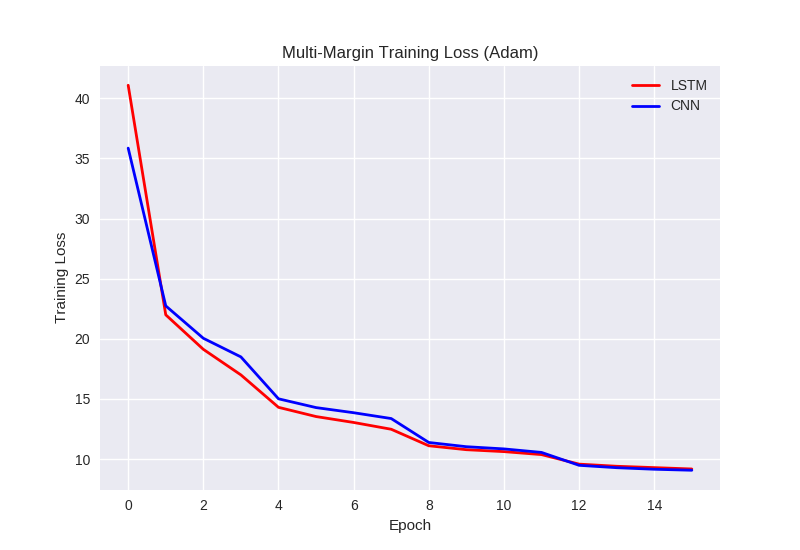
\includegraphics[width=0.55\columnwidth]{img/report_training_loss_part1}
    \captionof{figure}{Training loss over epochs}
    \label{fig:exp1_training}
&
   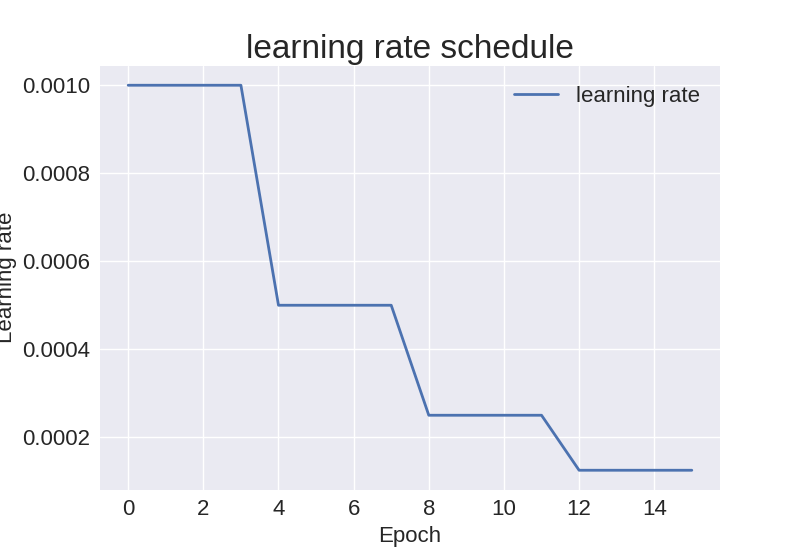
\includegraphics[width=0.55\columnwidth]{img/report_learning_rate_schedule.png}
   \captionof{figure}{Learning rate schedule over epochs}
   \label{fig:exp1_learning_rate}
   
&   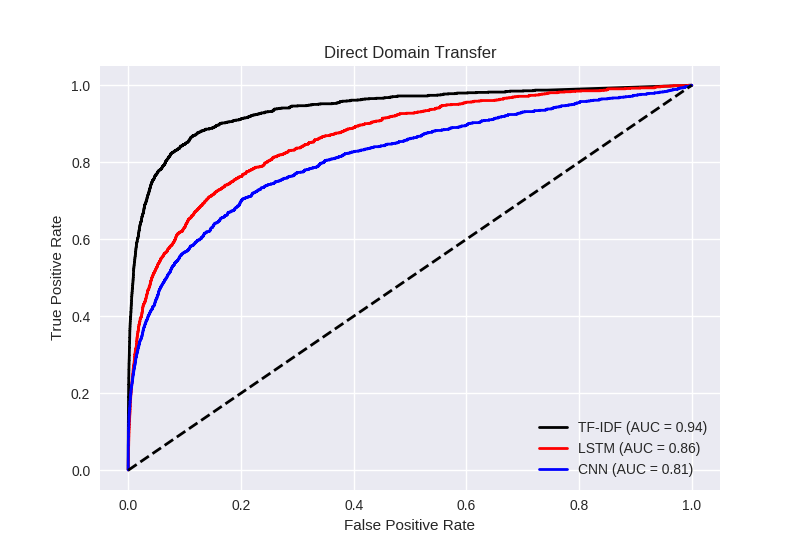
\includegraphics[width=0.55\columnwidth]{img/report_da_roc_direct}
    \captionof{figure}{ROC Direct transfer}
   \label{fig:exp2_roc_direct_transfer}
&
    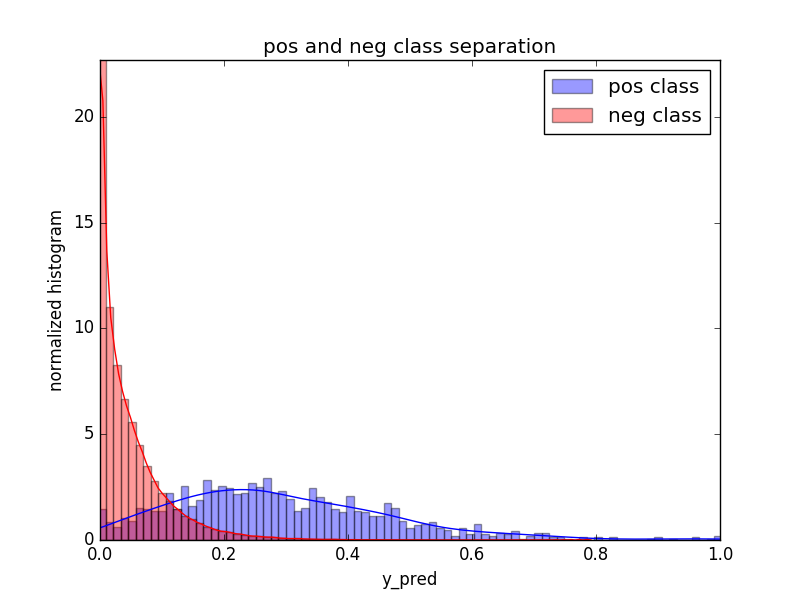
\includegraphics[width=0.55\columnwidth]{img/report_domain_transfer_tfidf_hist}
    \captionof{figure}{Direct transfer - class separation}
   \label{fig:exp2_direct_transfer}
 \\
    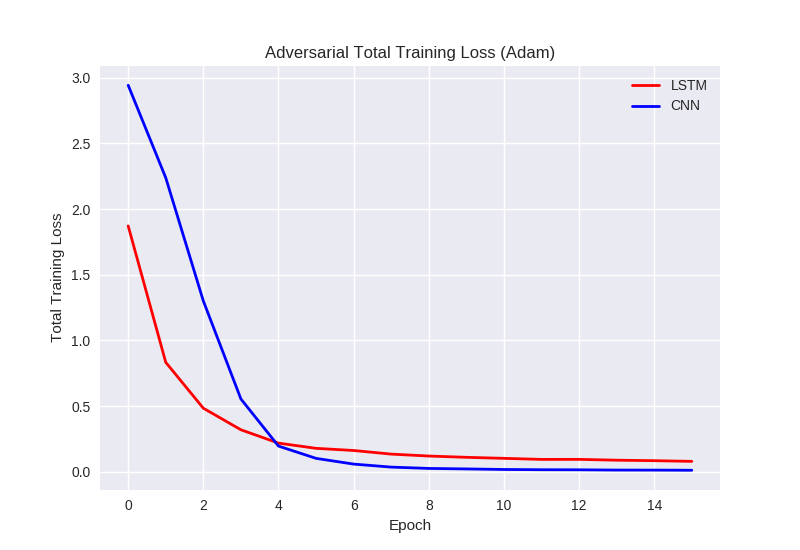
\includegraphics[width=0.55\columnwidth]{img/report_training_loss_adversarial_tot}
    \captionof{figure}{Total loss over epochs - Adversarial network}
    \label{fig:exp2_adversarial_loss_total}
&
   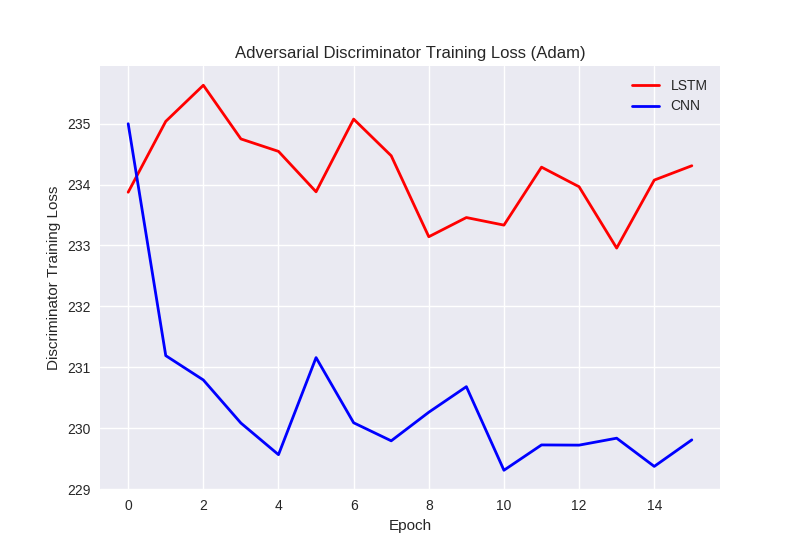
\includegraphics[width=0.55\columnwidth]{img/report_training_loss_adversarial_dis}
   \captionof{figure}{Loss of the discriminator network over epochs}
   \label{fig:exp2_adversarial_loss_discrimnator}
&
    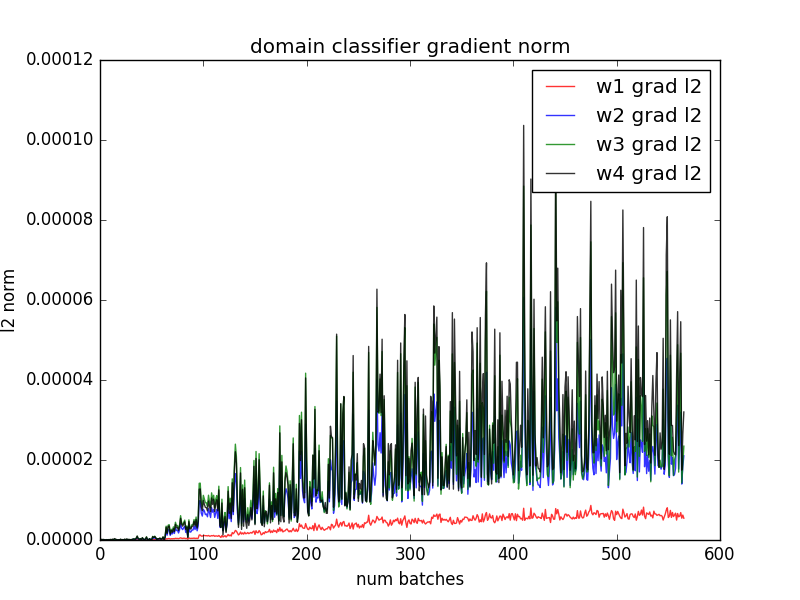
\includegraphics[width=0.55\columnwidth]{img/report_da_adversarial_gradient_norm}
    \captionof{figure}{Gradient norms - Domain classifier}
   \label{fig:exp2_gradient_norm}
   
&   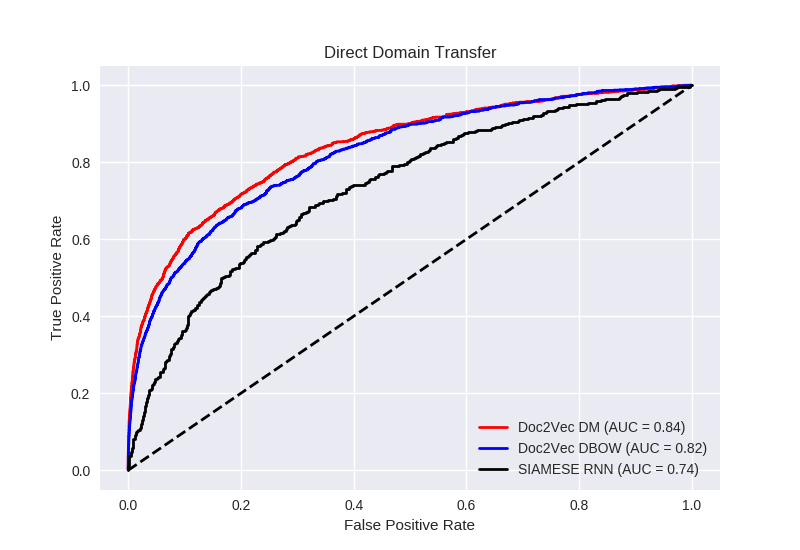
\includegraphics[width=0.55\columnwidth]{img/report_da_roc_part3.png}
    \captionof{figure}{Direct transfer - Experiment 3}
   \label{fig:exp3_siamese}

\end{tabularx}
\end{table*}


\subsection{Experiment 2}
Table \ref{tab:exp1} summarizes the performance of our models on the AUC(0.05) metric. The TF-IDF baseline transfer method has an AUC(0.05) score of 0.62. We see that the Direct-transfer CNN and LSTM baseline models perform better than the TF-IDF model by {\color{red}XX} points on an average. The neural models for domain adaptation clearly beat these two baselines by $0.10$ points on an average. These are encouraging results and demonstrate the robustness of the approach to domain adaptation.
Figure \ref{fig:exp2_roc_direct_transfer} shows direct domain transfer ROC AUC performance for the three baseline models - TF-IDF, LSTM and CNN. TF-IDF achieves highest direct transfer AUC. Figure \ref{fig:exp2_direct_transfer} shows the positive and negative class separation attained by the TF-IDF model. This histogram is normalized since the number of negative examples in the dataset far exceeds the number of positive (similar) question pairs. {\color{red}\st{We can see that by varying the threshold on the predicted label, we can attain the ROC curve shown on the left. Notice that the two classes are well-separated by the tf-idf model leading to a high AUC score.}}
Figure \ref{fig:exp2_adversarial_loss_total} shows the total adversarial training loss for the LSTM and CNN models. We see the difference in initialization of the two models by comparing the loss at epoch zero. The losses plateau after 8 epochs resulting in early stopping. Figure \ref{fig:exp2_adversarial_loss_discrimnator} shows the stochastic nature of the domain classifier loss. Its magnitude is much larger in comparison to the question encoder loss and therefore a small value of $\lambda$ ($1e$-$6$) is used to attenuate it. We found that AUC performance was very sensitive to the choice of $\lambda$. We selected the best value of lambda by sweeping between $1e$-$3$ to $1e$-$7$. We also examined the gradient norms of the domain classifier as shown in Figure \ref{fig:exp2_gradient_norm}. We found the gradient of the last among the 4 dense layers of the MLP to have be the highest and most stochastic. \st{The effect of the learning rate schedule on the MLP parameter weights can also be seen from the staircase in Figure. HAVE REMOVED THIS FIG OWING TO SPACE. NOT A LOT OF VALUE ADD}
\subsection{Experiment 3}
Figure \ref{fig:exp3_siamese} shows the ROC AUC performance of the Siamese RNN and \textsf{doc2vec} models. From Table \ref{tab:exp23}, we can see that the performance of these two techniques performs less favorably in comparison to adversarial domain transfer. Further, the DM architecture of \textsf{doc2vec} is slightly better in comparison to DBOW, which is also reported in the original paper \cite{doc2vec_paper}. The main difference between the Siamese RNN and the LSTM encoding network is the contrastive loss function and the additional dense layers introduced in the Siamese RNN network to aid in the domain transfer. We can see that direct transfer LSTM outperforms Siamese RNN suggesting that further optimization can be done to improve its performance.

\section{CONCLUSION}
We explore the task of question retrieval in online discussion forums. Given a question-answer pair, we employ neural techniques to detect similar such pairs on the forums. We find that neural techniques model this task well and outperform traditional IR-based approaches in finding similar content. Another area explored in this work is that of unsupervised domain transfer. Given a labeled dataset of question-answer pairs from a discussion forum on one topic, we evaluate how well neural approaches are able to transfer this knowledge of similarity detection onto question-answer pairs on another topic. No labeled information is available for the pairs on the new topic. We find that neural adversarial approaches to domain transfer perform better than baseline domain transfer approaches. We also explore other architectures for domain adaptation. We find that Siamese RNN, although suited for domain-adaptation-like tasks, does not perform as well as the adversarial setup. Further, \textsf{doc2vec} is unable to capture the feature-space which the adversarial network trains, rendering them unsuitable for this domain adaptation task. The simplicity in the architecture, the lack of any feature engineering required, and relatively low training time make adversarial neural models worthy of further study and possible adoption in industrial systems for such tasks. 

%ACKNOWLEDGEMENTS are optional
\section{Acknowledgements}
\label{ack}
The authors thank the course staff of 6.864, Fall 2017, MIT. This was a fun project!

%
% The following two commands are all you need in the
% initial runs of your .tex file to
% produce the bibliography for the citations in your paper.
\bibliographystyle{abbrv}
\bibliography{sigproc}  % sigproc.bib is the name of the Bibliography in this case
% You must have a proper ".bib" file
%  and remember to run:
% latex bibtex latex latex
% to resolve all references
%
% ACM needs 'a single self-contained file'!
%
%APPENDICES are optional
% SIGKDD: balancing columns messes up the footers: Sunita Sarawagi, Jan 2000.
% \balancecolumns

% That's all folks!
\end{document}
